% Diagrama de bloques del sistema completo (Tarea 2, pregunta 4).
\documentclass[border=4pt]{standalone}
% Estilo común de los diagramas: imita el tema por defecto de Mermaid usado en
% proyecto_1_grupal/docs/avance2/diagramas (nodos lavanda, grupos amarillos,
% etiquetas de flecha sobre gris, líneas punteadas para lo no permanente).
\usepackage[T1]{fontenc}
\usepackage[utf8]{inputenc}
\usepackage[scaled=0.95]{helvet}
\renewcommand{\familydefault}{\sfdefault}
\usepackage{amsmath}
\usepackage{tikz}
\usetikzlibrary{arrows.meta,positioning,fit,backgrounds,calc}
\definecolor{nodofondo}{HTML}{ECECFF}
\definecolor{nodoborde}{HTML}{9370DB}
\definecolor{grupofondo}{HTML}{FFFFDE}
\definecolor{grupoborde}{HTML}{AAAA33}
\definecolor{etiqueta}{HTML}{E8E8E8}
\definecolor{linea}{HTML}{333333}
\tikzset{
  every node/.style={text=linea},
  nodo/.style={draw=nodoborde, fill=nodofondo, line width=0.6pt, align=center,
    inner xsep=9pt, inner ysep=7pt, minimum height=13mm, font=\small},
  opcional/.style={nodo, dash pattern=on 4pt off 3pt, fill=black!3},
  flecha/.style={draw=linea, line width=0.6pt, -{Triangle[length=2.2mm,width=2mm]}},
  punteada/.style={flecha, dash pattern=on 4pt off 3pt},
  lbl/.style={fill=etiqueta, inner sep=2pt, align=center, font=\small},
  grupo/.style={draw=grupoborde, fill=grupofondo, line width=0.6pt, inner sep=7mm},
  titulo/.style={font=\small, anchor=north, inner sep=3pt},
}

\begin{document}
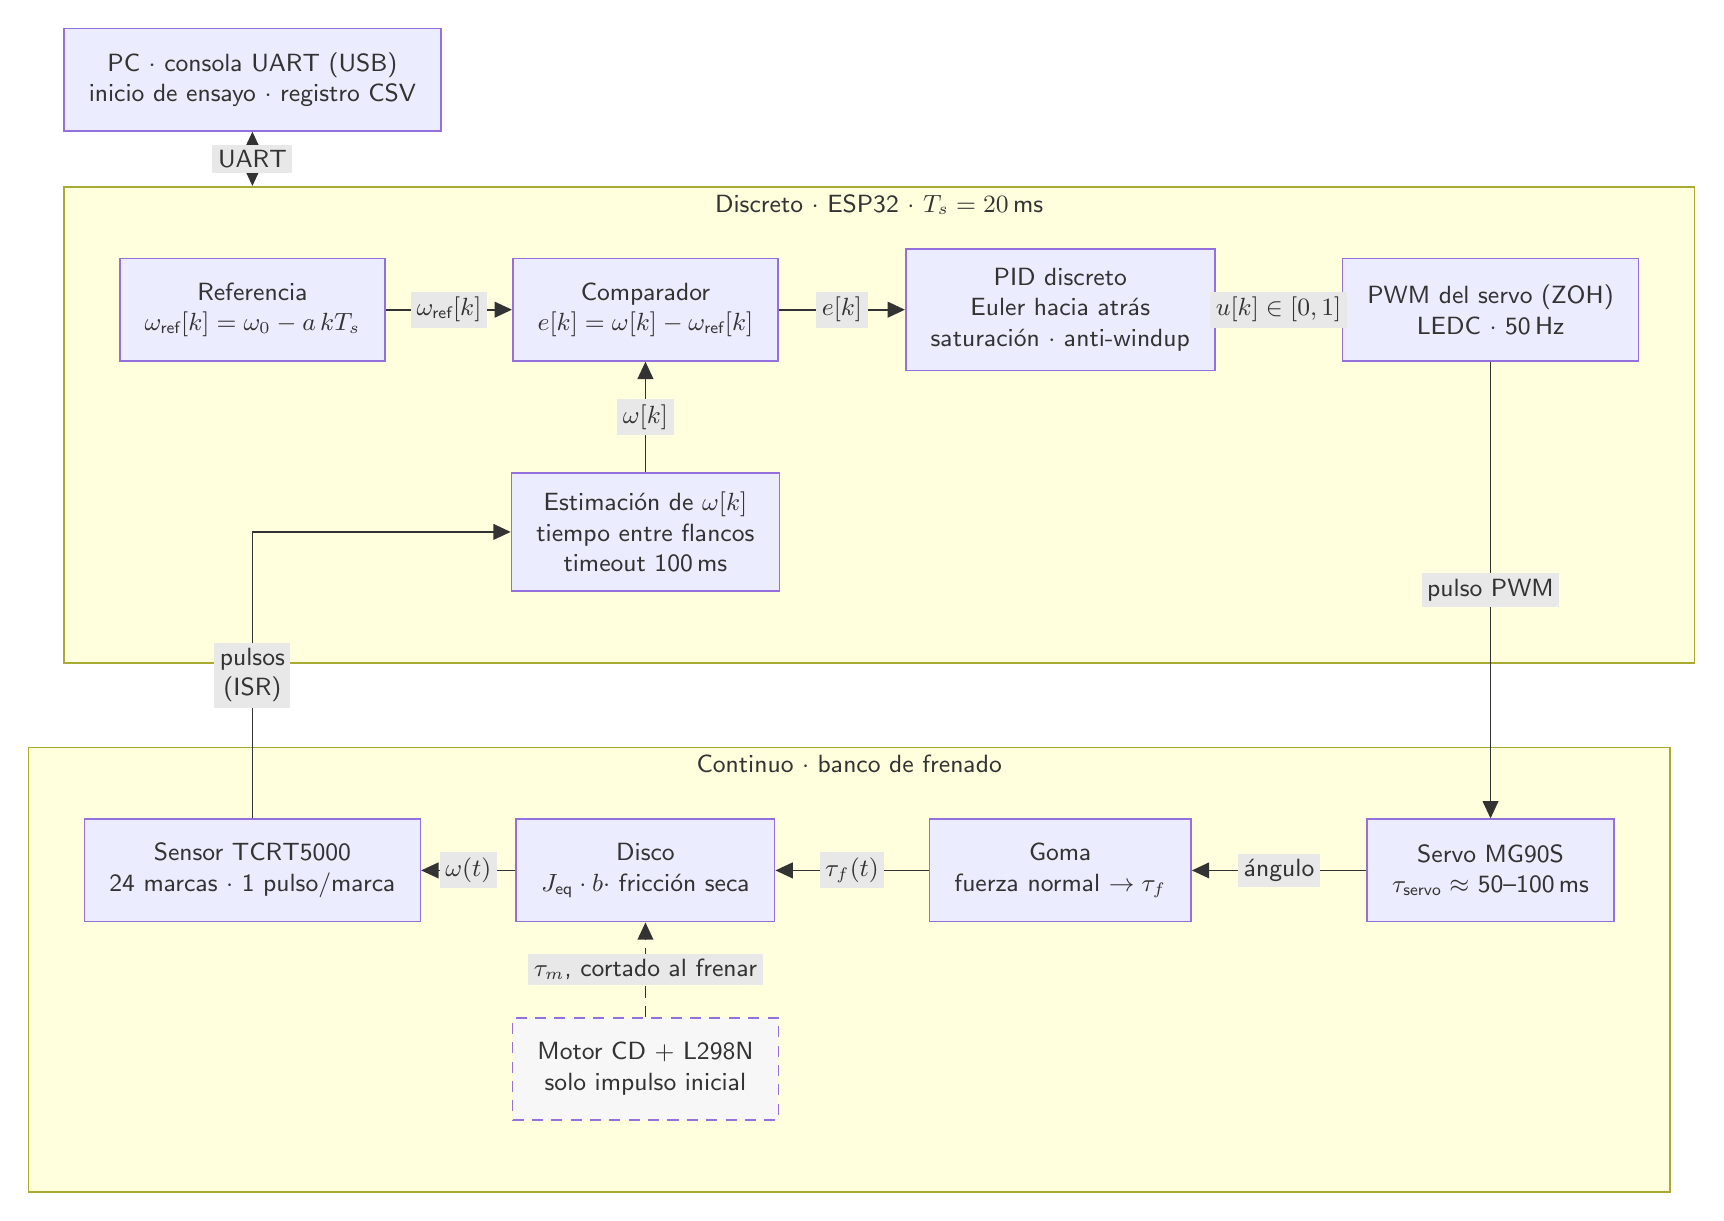
\begin{tikzpicture}[node distance=14mm]
  % Parte discreta: ESP32
  \node[nodo] (ref) {Referencia\\$\omega_\text{ref}[k]=\omega_0-a\,kT_s$};
  \node[nodo, right=16mm of ref] (cmp) {Comparador\\$e[k]=\omega[k]-\omega_\text{ref}[k]$};
  \node[nodo, right=16mm of cmp] (pid) {PID discreto\\Euler hacia atrás\\saturación $\cdot$ anti-windup};
  \node[nodo, right=16mm of pid] (pwm) {PWM del servo (ZOH)\\LEDC $\cdot$ 50\,Hz};
  \node[nodo, below=14mm of cmp] (est) {Estimación de $\omega[k]$\\tiempo entre flancos\\timeout 100\,ms};

  % Parte continua: banco de frenado
  \node[nodo, below=58mm of pwm] (servo) {Servo MG90S\\$\tau_\text{servo}\approx$ 50--100\,ms};
  \node[nodo] (goma) at (servo -| pid) {Goma\\fuerza normal $\rightarrow\tau_f$};
  \node[nodo] (disco) at (servo -| cmp) {Disco\\$J_\text{eq}\cdot b\cdot$ fricción seca};
  \node[nodo] (enc) at (servo -| ref) {Sensor TCRT5000\\24 marcas $\cdot$ 1 pulso/marca};
  \node[opcional, below=12mm of disco] (motor) {Motor CD + L298N\\solo impulso inicial};

  \node[nodo, above=16mm of ref] (pc) {PC $\cdot$ consola UART (USB)\\inicio de ensayo $\cdot$ registro CSV};

  \begin{scope}[on background layer]
    \node[grupo, fit=(ref)(pwm)(est), inner ysep=9mm] (gd) {};
    \node[titulo] at (gd.north) {Discreto $\cdot$ ESP32 $\cdot$ $T_s=20$\,ms};
    \node[grupo, fit=(enc)(servo)(motor), inner ysep=9mm] (gc) {};
    \node[titulo] at (gc.north) {Continuo $\cdot$ banco de frenado};
  \end{scope}

  \draw[flecha] (ref) -- node[lbl]{$\omega_\text{ref}[k]$} (cmp);
  \draw[flecha] (cmp) -- node[lbl]{$e[k]$} (pid);
  \draw[flecha] (pid) -- node[lbl]{$u[k]\in[0,1]$} (pwm);
  \draw[flecha] (est) -- node[lbl]{$\omega[k]$} (cmp);
  \draw[flecha] (pwm) -- node[lbl]{pulso PWM} (servo);
  \draw[flecha] (servo) -- node[lbl]{ángulo} (goma);
  \draw[flecha] (goma) -- node[lbl]{$\tau_f(t)$} (disco);
  \draw[flecha] (disco) -- node[lbl]{$\omega(t)$} (enc);
  \draw[flecha] (enc.north) |- node[lbl, pos=0.25]{pulsos\\(ISR)} (est.west);
  \draw[punteada] (motor) -- node[lbl]{$\tau_m$, cortado al frenar} (disco);
  \draw[flecha, {Triangle[length=2.2mm,width=2mm]}-{Triangle[length=2.2mm,width=2mm]}]
    (pc.south) -- node[lbl]{UART} (gd.north -| pc.south);
\end{tikzpicture}
\end{document}
